\documentclass[conference,a4paper]{IEEEtran}
\usepackage[T1]{fontenc}
\usepackage{graphicx}\usepackage{xcolor}\usepackage{tikz}
\usetikzlibrary{arrows.meta,positioning,calc}
\usepackage{url}\usepackage[hidelinks]{hyperref}
\setlength{\textfloatsep}{6pt plus 2pt minus 2pt}\setlength{\intextsep}{6pt plus 2pt minus 2pt}\setlength{\dbltextfloatsep}{6pt plus 2pt minus 2pt}
\newcommand{\orcidlogo}[1]{\IfFileExists{orcid.png}{\href{https://orcid.org/#1}{\raisebox{-0.10em}{\includegraphics[height=0.85em]{orcid.png}}}}{}}
\begin{document}
	\title{Operational Safety and Cybersecurity Assurance of AI-Based Perception in Highly Automated Driving}
	\author{
		\IEEEauthorblockN{Milin Patel\,\orcidlogo{0000-0002-8357-6018}}
		\IEEEauthorblockA{Institute for Driver Assistance and Connected Mobility\\ Kempten University of Applied Sciences\\ Benningen, Germany\\ milin.patel@hs-kempten.de}
		\and
		\IEEEauthorblockN{Rolf Jung\,\orcidlogo{0000-0002-0366-4844}}
		\IEEEauthorblockA{Faculty of Computer Science\\ Kempten University of Applied Sciences\\ Kempten, Germany\\ rolf.jung@hs-kempten.de}}
	\maketitle
	
	\begin{abstract}
		In 2026 the United Nations adopted the first global framework for fully driverless automated driving systems that bases approval on a safety case and obliges the manufacturer to monitor operation and report field occurrences. For an AI-based perception component this operational evidence is indirect, because runtime provides no ground truth against which a detection can be compared. Monitors report predictive uncertainty, distribution shift, and cybersecurity events instead. ISO 21448 (safety of the intended functionality), ISO/PAS 8800 (AI safety), and ISO/SAE 21434 (cybersecurity) each define a concern-specific operation-phase activity that uses this evidence. A runtime anomaly arrives without a concern label, because the same degraded detection can follow from a performance insufficiency or from an attack. This paper states one gap at the clause level: no clause in these standards assigns such an anomaly to a concern, and none states how the concern-specific activities resolve into a single judgment on the assurance argument. The gap therefore has two missing steps, assignment and resolution. The paper separates this gap from the anomaly-detection problem existing work addresses and specifies the requirements a method that closes it must satisfy, leaving the method to future work.
	\end{abstract}
	\begin{IEEEkeywords}
		assurance argument, safety case, cybersecurity, runtime monitoring, AI-based perception, automated driving
	\end{IEEEkeywords}
	
	\section{Introduction}
	This paper addresses assurance of AI-based perception in highly automated driving. In 2026 the UN World Forum for Harmonization of Vehicle Regulations (WP.29) adopted the first global framework for fully driverless automated driving systems; it bases approval on a safety case and requires a safety management system, in-service monitoring and reporting, and a data storage system \cite{UNECE2026}. Operation-phase evidence thus informs the safety case throughout deployment. For an AI-based perception component this evidence is indirect. Unlike a planning function, whose output can be checked at runtime against formalized traffic rules \cite{Maierhofer2020}, a perception function has no ground truth to check a detection against. In operation it produces monitor outputs: predictive uncertainty and ensemble disagreement \cite{PatelJungVEHITS2026}, distribution-shift indicators, and cybersecurity events \cite{ISO21434}. Re-evaluation is activated by a change in monitor output or by a software update; the framework provides for both triggers \cite{UNECE2026}.
	
	An assurance argument decomposes a top claim, that the item is acceptably safe and secure, into sub-claims supported by evidence; the safety case is the recorded form of that argument together with its evidence. Its sub-claims are organized by concern, that is, by the scope of one standard: safety of the intended functionality (SOTIF) under ISO~21448, AI safety under ISO/PAS~8800, and cybersecurity under ISO/SAE~21434.

	An anomaly in the operational evidence is an abnormal monitor output, for example, a scene region where detections drop. It carries no concern label and does not show whether the cause falls to SOTIF, AI safety, or cybersecurity. The same missing region follows from rain, sparse returns, or a rare object pose as a performance insufficiency under ISO~21448, and from a spoofing or relay attack as a cybersecurity event under ISO/SAE~21434 \cite{Sato2025}. Random hardware faults lie outside this ambiguity: ISO~26262 requires diagnostic mechanisms that label such a fault when it is detected \cite{ISO26262}, so it does not reach the argument unlabeled. The performance-insufficiency reading activates the SOTIF re-evaluation and, where the cause lies in the AI component itself, the AI-safety re-evaluation; the attack reading activates the cybersecurity re-evaluation (Fig.~\ref{fig:gap}). No clause assigns the anomaly to a concern, and no clause resolves the results of these activities into one judgment on whether the assurance argument still holds. We treat this as one gap with two missing steps: assignment, a precondition for any concern-specific activity to be the right one to act, and resolution, required for the separate results to reach the top claim. We are aware of no published incident that attributes a deployed automated-driving failure to this ambiguity. The motivation rests on the reporting duty \cite{UNECE2026}, a demonstrated on-road attack \cite{Sato2025}, and the absence of a method to separate the two causes \cite{Gao2022}. This paper takes the position that this gap is where operational assurance is left undefined, that it must be closed at the assurance argument where the concern-specific activities meet, and that closing it is an in-service re-evaluation of the safety case, not an in-vehicle runtime function. The paper specifies the requirements a method that closes the gap must satisfy.
	
	\begin{figure}[t]
		\centering
		\setlength{\abovecaptionskip}{4pt}
		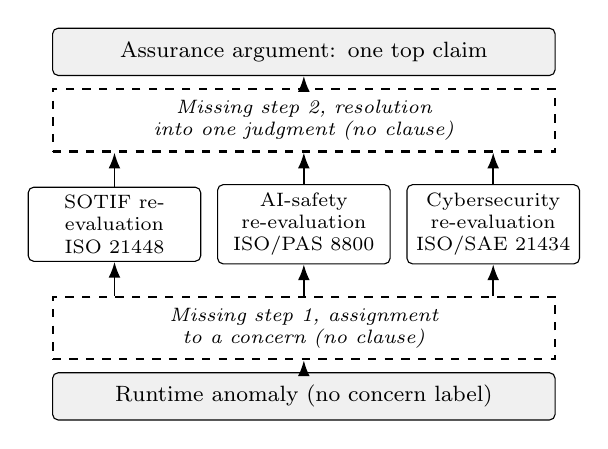
\begin{tikzpicture}[
			every node/.style={font=\footnotesize},
			io/.style={draw, rounded corners=2pt, fill=gray!12, align=center, inner sep=4pt, text width=6.1cm, minimum height=6mm},
			concern/.style={draw, rounded corners=2pt, fill=white, align=center, inner sep=3pt, font=\scriptsize, text width=1.98cm, minimum height=7.5mm},
			gap/.style={draw, dashed, thick, align=center, inner sep=4pt, font=\scriptsize\itshape, text width=6.1cm, minimum height=6mm},
			ar/.style={-{Latex[length=2mm]}, semithick}]
			\node[io] (top) {Assurance argument: one top claim};
			\node[gap, below=1.5mm of top] (res) {Missing step~2, resolution into one judgment (no clause)};
			\node[concern, below=4mm of res] (ai) {AI-safety re-evaluation\\ ISO/PAS 8800};
			\node[concern, left=2mm of ai] (sotif) {SOTIF re-evaluation\\ ISO 21448};
			\node[concern, right=2mm of ai] (sec) {Cybersecurity re-evaluation\\ ISO/SAE 21434};
			\node[gap, below=4mm of ai] (assign) {Missing step~1, assignment to a concern (no clause)};
			\node[io, below=1.5mm of assign] (anom) {Runtime anomaly (no concern label)};
			\draw[ar] (anom) -- (assign);
			\draw[ar] (assign.north -| sotif.south) -- (sotif.south);
			\draw[ar] (assign.north -| ai.south) -- (ai.south);
			\draw[ar] (assign.north -| sec.south) -- (sec.south);
			\draw[ar] (sotif.north) -- (res.south -| sotif.north);
			\draw[ar] (ai.north) -- (res.south -| ai.north);
			\draw[ar] (sec.north) -- (res.south -| sec.north);
			\draw[ar] (res) -- (top);
		\end{tikzpicture}
		\caption{Read upward from the evidence, as in an assurance-case notation. A single runtime anomaly can activate any of the concern-specific re-evaluations (solid, each defined by a standard). Assignment to a concern (missing step~1) and resolution into one judgment (missing step~2) are dashed because no clause defines them; they sit between the operational evidence and the top claim that evidence is meant to support.}
		\label{fig:gap}
	\end{figure}
	
	\section{Operation-Phase Activity Defined by Each Standard}
	\begin{table}[t]
		\caption{Operation-phase activity defined by each standard, and the element each leaves undefined}
		\label{tab:standards}
		\centering\scriptsize
		\renewcommand{\arraystretch}{1.1}
		\begin{tabular}{@{}p{1.75cm}p{2.75cm}p{2.75cm}@{}}
			\hline
			\textbf{Standard} & \textbf{Operation-phase activity defined} & \textbf{Element not defined}\\
			\hline
			ISO 21448 (SOTIF) & SOTIF argument on a field result (Clause 13.4) & Result-to-argument mapping\\
			ISO/PAS 8800 (AI safety) & AI-safety argument; re-evaluate after change & Which evidence re-opens which element\\
			ISO/SAE 21434 (cybersecurity) & Monitor, evaluate, treat & Re-evaluation of the case; change management scoped to requirements\\
			\hline
			\multicolumn{3}{@{}p{7.35cm}@{}}{None of these standards assigns an unlabeled anomaly to a concern (missing step~1), or resolves the concern-specific results into one judgment on the assurance argument (missing step~2).}\\
			\hline
		\end{tabular}
	\end{table}
	The pattern in Table~\ref{tab:standards} is uniform in scope: each activity is defined within one concern and produces a result for that concern alone. ISO/SAE~21434 differs in endpoint. Its continual monitoring ends in risk treatment, and no clause re-evaluates the cybersecurity case \cite{ISO21434}. The activities converge only at the assurance argument, where the SOTIF, AI-safety, and cybersecurity claims sit under one top claim, the top of the safety case \cite{ISO21448,ISOPAS8800,PatelJungWAISE2026}.
	
	\section{Assignment and Resolution of the Anomaly}
	The anomaly has one form in the data and two candidate causes, a performance insufficiency or an attack. A 2022 survey of autonomous-driving security reports no method that distinguishes the two from the readings alone: abnormal sensor readings can originate from an attack or from a non-malicious cause, and multi-sensor cross-validation detects an anomaly without assigning it to a cause \cite{Gao2022}. Processing the anomaly within one concern presupposes an assignment that no clause performs. Without it, the re-evaluations can all act and produce results with no rule to combine them. Each can instead treat the anomaly as another's responsibility, so none acts. ISO~21448, in Clause 1 and Table 1, excludes cybersecurity threats and refers an attack to ISO/SAE~21434, while ISO/SAE~21434 does not address performance insufficiency \cite{ISO21434,ISO21448}. They can also reach opposed results, one keeping its concern's claim while another withdraws it.
	
	The first step alone would not close the gap. With every anomaly labeled, the concern-specific results still meet at the top claim, where the evidence has different measurement scales, such as a calibrated probability, an ensemble disagreement value, a binary event indicator, or a risk rating, and no rule combines them. Operation adds conditions that design-time analysis does not face: evidence that arrives asynchronously, a component that changes under updates, and a reporting obligation that requires a current judgment on demand \cite{UNECE2026}.
	
	\section{Relation to Existing Work}
	Machine-learning assurance guidance provides an AI argument structure not linked to the automotive standards' clauses \cite{Hawkins2021}, and dynamic safety cases stay within the safety concern \cite{Denney2015}. Across concerns, an argument-pattern method structures them at design time without defining how runtime evidence is interpreted \cite{Warg2019}, and a co-assurance framework leaves cross-concern operational evidence as an open problem \cite{JohnsonKelly2018}. A runtime method distinguishes attack from fault using branches already labeled attack or fault in a fault tree, not at the assurance argument \cite{Cardoso2022}. None assigns a runtime monitor output across concerns and then resolves the concern-specific results into one judgment on the argument.
	
	\section{The Position: Requirements for a Method that Closes the Gap}
	The concern-specific activities have no shared procedure or output below the argument \cite{PatelJungWAISE2026}. A method placed below that point reproduces the assignment problem within one concern. Each requirement below follows from one feature of the gap; each is necessary, and we do not claim the set is sufficient. \textbf{R1, heterogeneous evidence:} accept evidence with different measurement scales at one claim without imposing a common scale that no source standard defines. \textbf{R2, assignment:} contain an assignment step for an unlabeled anomaly, and treat the unassignable case as a defined outcome with a stated effect on the judgment. \textbf{R3, traceability and currency:} produce a judgment traceable to the operation-phase activities in ISO~21448, ISO/PAS~8800, and ISO/SAE~21434, current with respect to evidence that arrives asynchronously, and reportable under the in-service obligation \cite{UNECE2026}. \textbf{R4, modification:} state which evidence remains valid after a component update and which is re-opened, consistent with the modification provisions of ISO/PAS~8800 and ISO~26262 \cite{ISO26262}. A candidate direction treats the anomaly as a defeater of the top claim, that is, a doubt that invalidates the claim unless it is eliminated, following eliminative argumentation \cite{Bloomfield2024}: assignment attaches the defeater to a concern's sub-claim, resolution propagates its status to the top claim, an unresolved defeater is R2's residual outcome, and defeaters combine as claim status rather than on a common scale, as R1 requires. Whether this satisfies R1--R4 in full, and how to benchmark it, remain open.
	
	\section{Implications for Industry and Standardization}
	Under the WP.29 framework a manufacturer reports field occurrences against a safety case fixed at approval, with no defined procedure to turn a field anomaly into a current judgment on that case, on which continued operation depends \cite{UNECE2026}. The gap identifies what a revised ISO/PAS~8800 and ISO/SAE~21434 could add: an assignment step and a resolution step at the interface among the concern-specific activities. We expect the same gap wherever one component is assured against several concern-specific standards.
	
	\begin{thebibliography}{15}
		\scriptsize\setlength{\itemsep}{0pt}\setlength{\parskip}{0pt}
		\bibitem{UNECE2026} UNECE, ``UNECE adopts first-ever global rules allowing fully autonomous vehicles,'' World Forum for Harmonization of Vehicle Regulations (WP.29), doc.\ ECE/TRANS/WP.29/2026/139, Geneva, 24~Jun.\ 2026.
		\bibitem{PatelJungVEHITS2026} M. Patel and R. Jung, ``Uncertainty evaluation to support safety of the intended functionality analysis for identifying performance insufficiencies in ML-based LiDAR object detection,'' in \emph{Proc. VEHITS}, SciTePress, 2026.
		\bibitem{ISO21434} ISO/SAE, ``Road vehicles: Cybersecurity engineering,'' ISO/SAE 21434:2021.
		\bibitem{Sato2025} T. Sato et al., ``On the realism of LiDAR spoofing attacks against autonomous driving vehicle at high speed and long distance,'' in \emph{Proc. NDSS}, 2025.
		\bibitem{Gao2022} C. Gao, G. Wang, W. Shi, Z. Wang, and Y. Chen, ``Autonomous driving security: state of the art and challenges,'' \emph{IEEE Internet of Things J.}, vol. 9, no. 10, pp. 7572--7595, 2022.
		\bibitem{ISO21448} ISO, ``Road vehicles: Safety of the intended functionality,'' ISO 21448:2022.
		\bibitem{ISOPAS8800} ISO, ``Road vehicles: Safety and artificial intelligence,'' ISO/PAS 8800:2024.
		\bibitem{PatelJungWAISE2026} M. Patel and R. Jung, ``Integrating cybersecurity into the AI safety assurance argument: a GSN pattern for AI-based perception components in highly automated driving,'' in \emph{SafeComp 2026 Workshops (WAISE)}, LNCS, Springer, 2026, in press.
		\bibitem{Hawkins2021} R. Hawkins, C. Paterson, C. Picardi, Y. Jia, R. Calinescu, and I. Habli, ``Guidance on the Assurance of Machine Learning in Autonomous Systems (AMLAS),'' Univ. of York, 2021.
		\bibitem{Denney2015} E. Denney, G. Pai, and I. Habli, ``Dynamic safety cases for through-life safety assurance,'' in \emph{Proc. IEEE/ACM ICSE}, vol. 2, pp. 587--590, 2015.
		\bibitem{Warg2019} F. Warg and M. Skoglund, ``Argument patterns for multi-concern assurance of connected automated driving systems,'' in \emph{Proc. CERTS}, OASIcs 73, pp. 3:1--3:13, Schloss Dagstuhl, 2019.
		\bibitem{JohnsonKelly2018} N. Johnson and T. Kelly, ``An assurance framework for independent co-assurance of safety and security,'' \emph{J. System Safety}, vol. 54, no. 3, pp. 32--38, 2018.
		\bibitem{Cardoso2022} R. C. Cardoso, A. Ferrando, and M. Fisher, ``Extending attack-fault trees with runtime verification,'' \emph{EPTCS}, vol. 371, pp. 193--207, 2022.
		\bibitem{ISO26262} ISO, ``Road vehicles: Functional safety,'' ISO 26262:2018, Parts 1--12.
		\bibitem{Bloomfield2024} R. Bloomfield and J. Rushby, ``Confidence in Assurance 2.0 cases,'' in \emph{The Practice of Formal Methods}, LNCS 14780, Springer, 2024, pp. 1--23.
		\bibitem{Maierhofer2020} S. Maierhofer, A.-K. Rettinger, E. C. Mayer, and M. Althoff, ``Formalization of interstate traffic rules in temporal logic,'' in \emph{Proc. IEEE Intelligent Vehicles Symp. (IV)}, 2020, pp. 752--759.
	\end{thebibliography}
\end{document}